\begin{frame}
    \frametitle{¿Por qué NoSQL?}

    Pero, ¿por qué surgen las bases de datos no relacionales?

     
    
    Principalmente por el crecimiento exponencial de la información, debido al uso de nuevas tecnologías en la sociedad.
    
     
    
    Dicho crecimiento es impulsado por

     
    
    \begin{itemize}
        \item Internet             
        \item Teléfonos móviles     
        \item Redes Sociales         
        \item etc.                   
    \end{itemize}

    Como consecuencia surgieron conceptos como

     

    \begin{itemize}
        \item Web 2.0
        \item Big Data
        \item Cloud Computing
    \end{itemize}
\end{frame}

\begin{frame}
    \frametitle{¿Por qué NoSQL?}

    Estos avances llevaron tanto a la industria como a la academia a replantearse el uso de los modelos relacionales debido a sus limitaciones naturales en el manejo de grandes cantidades de información.

     
    
    Se necesitaban (\textit{necesitan}) sistemas que escalen horizontalmente de manera sencilla.
    
     

    Se empiezan a investigar y desarrollar posibles alternativas por fuera de los modelos relacionales, que resuelvan estos problemas.
    
     

    Prinpalmente es por esto que surgen las \textit{Bases de Datos NoSQL}.
\end{frame}

\begin{frame}
    \frametitle{¿Por qué NoSQL? - Tecnologías vs NoSQL}

    \centering
    
    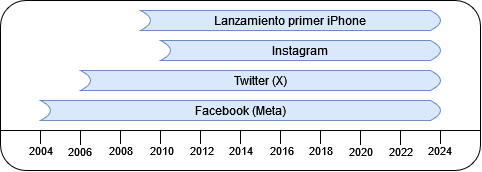
\includegraphics[width=0.65\textwidth]{diagramas/linea-temporal-tecno.png}

    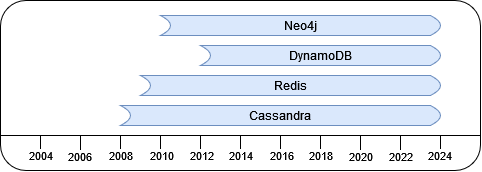
\includegraphics[width=0.65\textwidth]{diagramas/lineatemporal-nosql.png}
\end{frame}